\documentclass[main.tex]{subfiles}
\begin{document}
Các bạn có thể copy nội dung của các đoạn code trong phần này ở link sau: 
%%%%%%%%%%%%%%%%%%%%%%%%%%%%%%%%%%%%%%%%%%%%%
\subsection{Con trỏ cơ bản}
\textit{Lưu ý: các địa chỉ của các ô nhớ trong những hình dưới đây chỉ mang tính chất minh hoạ}.

\subsubsection{Câu a}
Do \code{p} là một con trỏ, trỏ đến \code{a} nên \code{*p} chính là \code{a}. Phép gán \code{*p += 4} tương đương \code{a += 4} nên đáp án là \code{19.75}.

\subsubsection{Câu b}
Do \code{p} trỏ đến cùng vùng nhớ với \code{a}, nên các thao tác truy xuất bộ nhớ thông qua \code{p} cũng hoàn toàn tương tự với các thao tác truy xuất bộ nhớ thông qua \code{a}.

\begin{center}
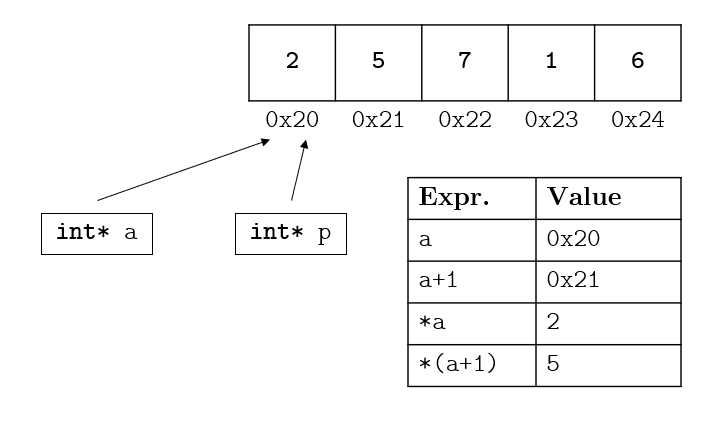
\includegraphics[width=0.7\textwidth]{image/ans_CTRLCB_b.png}
\end{center}

Ta thấy \code{*(p+1)} trùng với \code{*(a+1)}, chính là \code{a[1]}. Còn \code{*a} chính là \code{a[0]}, có giá trị là \code{2}.\\
Vậy \code{*(p + 1) += *a;} tương đương với phép gán \code{a[1] += a[0]}.\\
Tương tự, \code{cout << *(a + 1);} là \code{cout << a[1]}, nên kết quả in ra màn hình sẽ là \code{7}.

\subsubsection{Câu c}
\begin{figure}[H]
\centering
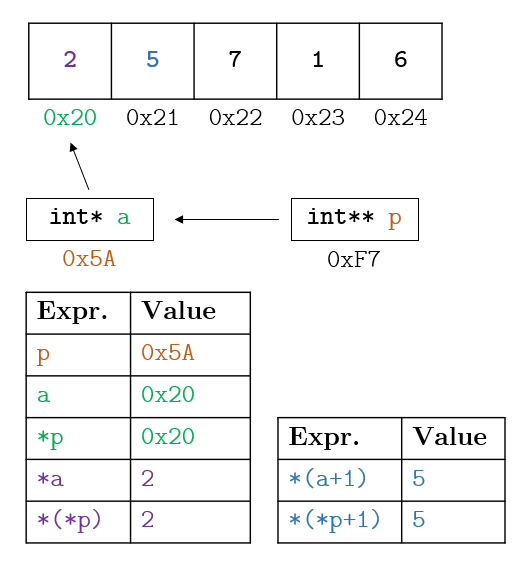
\includegraphics[width=0.5\textwidth]{image/ans_CTRLCB_c.png}
\end{figure}

Do \code{p} là một con trỏ, trỏ đến \code{a} nên \code{*p} chính là \code{a}. \\
\code{(*p)[4]} tương đương với \code{a[4]}, \code{*(*p + 1)} tương đương với \code{*(a + 1)}, chính là \code{a[1]}. Tự suy luận, ta có kết quả là \code{7}.

\subsubsection{Câu d}
Ta thấy \code{*(a+2)} chính là \code{a[2]}. \\
Nếu ta đặt \code{u = *(a+2)} thì \code{(*(a+2)+1)} sẽ trở thành \code{*(u+1)}, chính là \code{u[1]}.\\
Mà vì \code{u = *(a+2) = a[2]} nên \code{u[1]} chính là \code{a[2][1]}.\\
Giá trị tại vị trí \code{a[2][1]} chính là \code{1}.

Trên đây là một cách giải thích theo phong cách ``toán học''. Nếu các bạn muốn một cách giải thích theo bản chất của con trỏ có thể tham khảo hình dưới đây (tự tham khảo):
\begin{figure*}
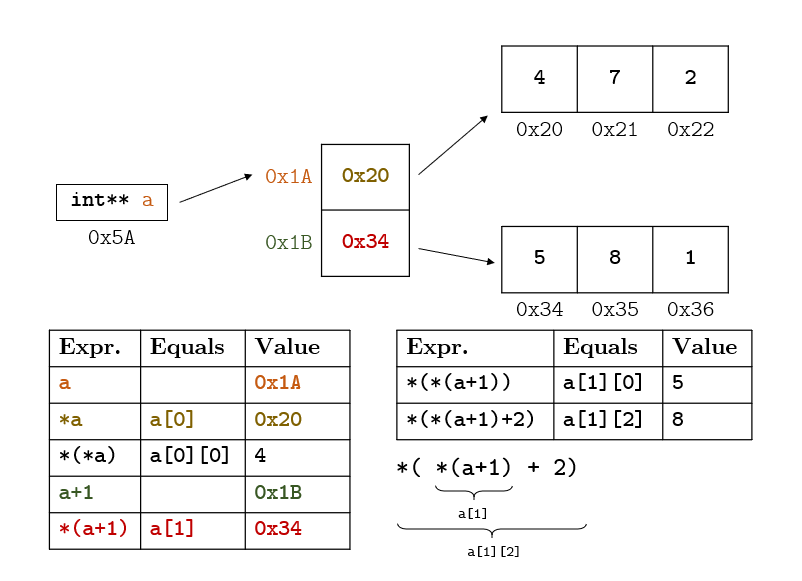
\includegraphics[width=0.6\textwidth]{image/ans_CTRLCB_d.png}
\end{figure*}

%%%%%%%%%%%%%%%%%%%%%%%%%%%%%%%%%%%%%%%%%%%%%

\subsection{Con trỏ nâng cao}
\subsubsection{Câu a}
\inputminted[linenos]{cpp}{answer_sources/ConTroNC_a.cpp}

\subsubsection{Câu b}
Nhắc lại kiến thức về con trỏ 2 cấp:\\
\begin{figure*}
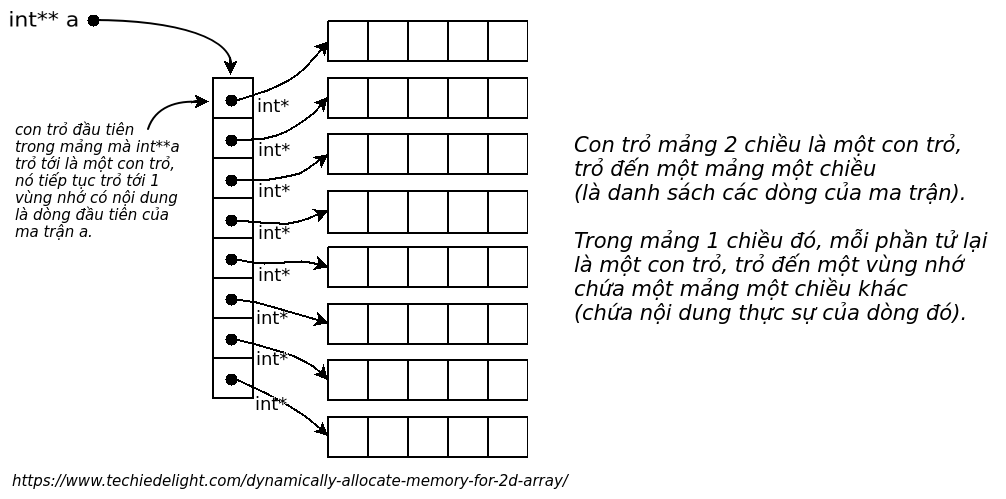
\includegraphics[width=1\textwidth]{image/ans_CTRLNC_1.png}
\end{figure*}

\inputminted[linenos]{cpp}{answer_sources/ConTroNC_b.cpp}
\textit{Lưu ý: Ta phải giải phóng các phần tử của a trước khi giải phóng a, vì bản thân a chỉ là một con trỏ 2 cấp, nó không thực sự chứa nội dung của ma trận. Khi ta giải phóng a thì các con trỏ thành phần bên trong a vẫn còn tồn tại, gây rò rỉ bộ nhớ nếu như ta không giải phóng trước.}

\begin{center}
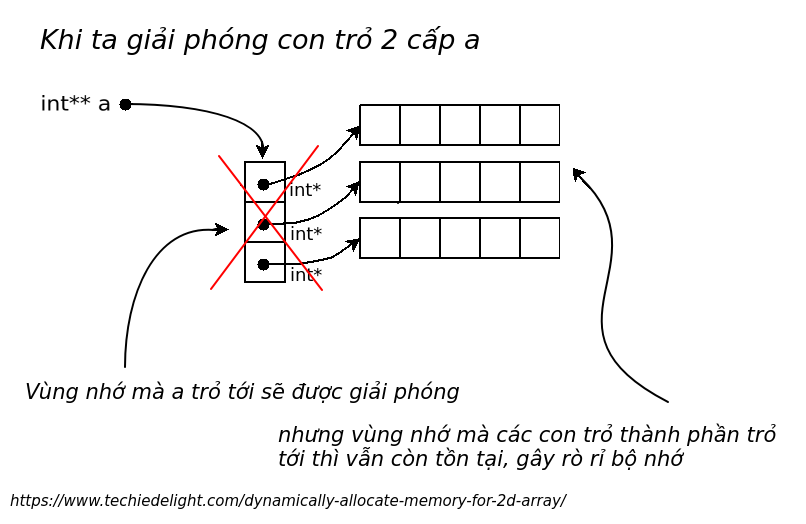
\includegraphics[width=0.8\textwidth]{image/ans_CTRLNC_2.png}
\end{center}


\subsubsection{Câu c}
\inputminted[linenos]{cpp}{answer_sources/ConTroNC_c.cpp}

%%%%%%%%%%%%%%%%%%%%%%%%%%%%%%%%%%%%%%%%%%%%%

\subsection{Danh sách liên kết}
\inputminted[linenos]{cpp}{answer_sources/DanhSachLK.cpp}

%%%%%%%%%%%%%%%%%%%%%%%%%%%%%%%%%%%%%%%%%%%%%

\subsection{Ngăn xếp, hàng đợi}
\subsubsection{Ngăn xếp}
Ta để ý là các cặp dấu ngoặc xuất hiện theo thứ tự 
first in first out, có nghĩa là dấu mở ngoặc nào tới sau thì nó phải được đóng trước. Do đó ta sử dụng stack để giải bài toán này. Cụ thể như sau:
\begin{itemize}
    \item Ta duyệt qua từng kí tự của chuỗi đó.
    \item Nếu ta gặp một dấu mở ngoặc, ta đẩy nó vào stack.
    \item Nếu ta gặp một dấu đóng ngoặc, ta kiểm tra thử nó có cùng loại với dấu mở ngoặc mà ta gặp gần nhất hay không (dấu mở ngoặc gần nhất là phần tử trên đỉnh stack). Nếu có, ta tiếp tục xét kí tự tiếp theo. Nếu khác loại thì coi như chuỗi là không hợp lệ (trường hợp này là bị thiếu dấu mở ngoặc, dư dấu đóng ngoặc).
    \item Sau khi duyệt hết các kí tự trong chuỗi, ta kiểm tra xem trong stack còn dư phần tử nào hay không, nếu có thì ta đã rơi vào trường hợp dư dấu mở ngoặc, thiếu dấu đóng ngoặc.
    \item Nếu chuỗi nhập vào không vi phạm bất cứ tiêu chuẩn nào thì nó là hợp lệ.
\end{itemize}

\inputminted[linenos]{cpp}{answer_sources/Stack.cpp}

%%%%%%%%%%%%%%%%%%%%%%%%%%%%%%%%%%%%%%%%%%%%%

\subsubsection{Hàng đợi}

%%%%%%%%%%%%%%%%%%%%%%%%%%%%%%%%%%%%%%%%%%%%%

\subsection{Đệ quy}
Chưa soạn

\subsection{Quy hoạch động}
Chưa soạn

%%%%%%%%%%%%%%%%%%%%%%%%%%%%%%%%%%%%%%%%%%%%%

\subsection{Bài tập tự luyện ở nhà}
Lưu ý: trong file pdf, phần giải thích này chỉ có giải thích, không có code. Các bạn vui lòng vào link được đính kèm ở đầu section để xem code.
\subsubsection{Cấp phát động}
Không có gì phải giải thích nhiều, thực hiện tương tự như khi thao tác với ma trận số nguyên.
Cần lưu ý khi truyền một con trỏ trỏ đến kiểu dữ liệu \code{T} vào hàm, mà ta muốn thay đổi giá trị của con trỏ đó (như cấp phát hay xoá) thì ta cần phải truyền dưới dạng tham chiếu: 
\begin{minted}{cpp}
void foo(T* &ptr) {
    ptr = new T[n];
    delete[] ptr;
}
\end{minted}
Hoặc dưới dạng tham trỏ
\begin{minted}{cpp}
void foo(T** ptr) {
    *ptr = new T[n];
    delete[] *ptr;
}
\end{minted}

%--------------------------------------------%
\subsubsection{Ngăn xếp}
\textbf{Nhắc lại về 2 cấu trúc:}
\begin{itemize}
    \item Stack: phần tử nào vào sau thì ra trước (như một chồng dĩa).
    \item Queue: phần tử nào vào sau thì ra sau (như một hàng người đợi mua trà sữa).
\end{itemize}

\textbf{Để implement một queue bằng 2 stack, ta có thể làm như sau}:
\begin{itemize}
    \item Giả sử ta có 2 stack gọi là stack (1) và stack (2).
    \item Khi push một phần tử vào queue, ta push vào (1).
    \item Khi muốn xem một phần tử ở đầu queue, vì phần tử ở đầu queue lại nằm dưới đáy của stack (1), nên ta pop tất cả phần tử từ stack (1) và chuyển qua stack (2). Lúc này, phần tử ở đầu queue đã nằm trên đỉnh của stack (2). Sau khi xem xong thì ta lại pop tất cả phần tử từ stack (2) bỏ về stack (1).
    \item Khi muốn xóa một phần tử khỏi queue, ta cũng chuyển tất cả phần tử từ (1) sang (2), nhưng sau đó phải bỏ phần tử trên đỉnh của stack (2) đi, rồi mới chuyển về lại stack (1).
\end{itemize}

\textbf{Ảnh động minh hoạ:}
\begin{itemize}
    \item Link ảnh GIF xem đỉnh queue: \href{https://ibb.co/64Hv1bH}{https://ibb.co/64Hv1bH}
    \item Link ảnh GIF xóa đỉnh queue: \href{https://ibb.co/syPCBFS}{https://ibb.co/syPCBFS}
\end{itemize}

\textbf{ Tối ưu hóa:}
Vì mỗi lần xem đỉnh queue ta phải pop (1) bỏ sang (2) rồi lại phải bỏ về (1), do đó ta nên tạo một biến tên là \code{top} bên trong struct queue của chúng ta để lưu giá trị của đỉnh queue để truy xuất thuận tiện hơn. Biến này sẽ được cập nhật giá trị khi và chỉ khi:
\begin{itemize}
    \item Khi queue đang rỗng mà chúng ta thêm một phần tử mới vào, thì phần tử đó sẽ là đỉnh của queue (các phần tử khác sau đó nằm ở phía sau phần tử đầu).
    \item Khi ta pop đỉnh của queue mà trong queue vẫn còn dữ liệu thì đỉnh queue sẽ là phần tử ngay kế sau.
\end{itemize}
%--------------------------------------------%


\end{document}